%% Einleitung.tex
%% $Id: einleitung.tex 61 2012-05-03 13:58:03Z bless $
%%

\chapter{Auswahl der Applikationen}
\label{ch:Apps}
%% ==============================
Unsere Auswahl der Apps
Erläuterung, Einführung
Bla fasel\ldots



%% ==============================
\section{Moves}
%% ==============================
\label{ch:Apps:sec:Moves}

Die Aktivitäts- und Location-Tracking App **Moves** soll ein automatisches Tagebuch sein, dass dem Nutzer sagt und zeigt, wo, wann und vor allem wie lang er in Bewegung war.

Dafür analysiert die App automatisch alle Lauf-, Radfahr- und Rennaktivität, nimmt Sie auf und speichert sie. 

Die gespeicherten Daten, wie z.B. die Distanz, die Dauer und die Anzahl der Schritte  sowie der Kalorienverbrauch jeder Aktivität, werden grafisch für den Benutzer übersichtlich dargestellt. 

Damit die App die Daten generieren kann ist sie „Always-On“ – also ständig mit dem Internet verbunden und es ist nicht nötig, die App zu Starten oder zu beenden.

Die einzelnen Funktionen der App sind: 

\subsection{Der Schrittzähler}

Der Schrittzähler in **Moves** ist die Hauptfunktion der App und zeigt dem Nutzer, wie viele Schritte er täglich gegangen ist. 

**Moves** nimmt neben dem normalen Laufen auch Fahrradfahren, Joggen oder die Fahrten mit anderen Verkehrsmitteln zu Kenntnis. 

Laut der App sind täglich 10.000 Schritte das Minimum, das ein gesundheitsbewusster Mensch erreichen sollte.

\begin{figure}[H]
\centering
	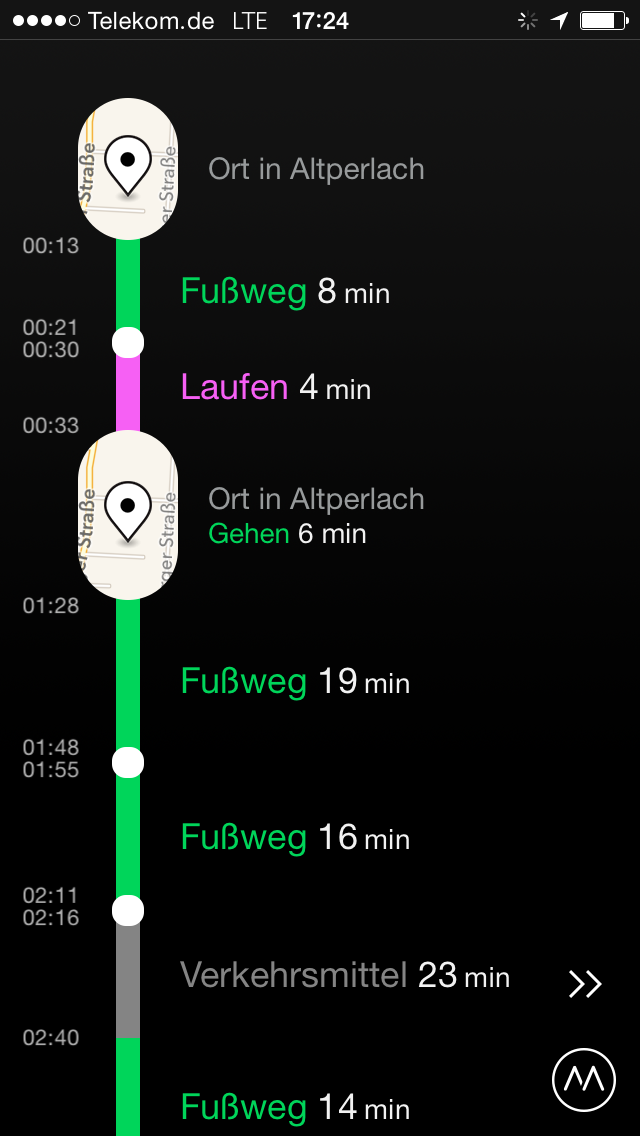
\includegraphics[width=0.6\textwidth]{images/moves_app_screenshot} 
	\caption[Screenshot des Moves Bildschirms]{Screenshot des Moves Bildschirms}
	\label{fig:moves_screenshot}
\end{figure}

\subsection{Der Kalorienzähler}

Mit dem Kalorienzähler der in der App zusätzlich beinhaltet ist, werden die Kalorien ermittelt, die in der jeweiligen Aktivität verbrannt wurden. 
Dazu kann dem Nutzer die tägliche optimale Menge der zu verbrennenden Kalorien angezeigt werden.

\subsection{Third-Party-Apps-Integration}

Da die App nicht nur die eigenen Dienste unterstützt, sondern auch Apps und Services von Drittanbietern. 
So existieren seit Kurzem die Möglichkeit, bis zu 15 andrere Apps in Moves zu integrieren. 
Der Start der API, die es Entwicklern und Anbietern von Third-Party-Services bzw. –Apps erlaubt, **Moves** einzubinden, war der erste Schritt, um die gesammelten Daten umfassend analysieren und auswerten zu können.

%% ==============================
\section{Hueman}
%% ==============================
\label{ch:Apps:sec:Hueman}

Beschreibung von Hueman

Bla fasel\ldots

%% ==============================
\section{Sleep Cycle}
%% ==============================
\label{ch:Apps:sec:SleepCycle}

Sleep Cycle ist Bio-Wecker, welcher das Schlafmuster des Benutzers analysiert und in der leichtesten Phase des Schlafes aufweckt.
Dafür zeichnet die Software die Bewegungsaktivitäten während des Schlafes auf und wertet diese aus.
Darüber hinaus biete die App zusätzliche Möglichkeiten um die Schlafgewohnheiten zu Kategorisieren sowie die Auswirkungen in unterschiedliche Charts zu begutachten. 

\subsection{Hintergrundwissen}
\label{ch:Apps:sec:Sleepcycle:subsec:H}

Der Schlaf ist ein wichtiges aktiver Teiles des täglichen Lebens und dient der Erholung von Körper und Geist.
Bei zu wenig Schlaf leidet der Körper unter Schlafmangel und kann zu Depressionen, Bluthochdruck oder weiteren Krankheiten führen. \cite{Chen:SleepMonitoring}

Das bereits ca. 15\% der Bevölkerung in Deutschland an immer wiederkehrenden Schlafstörungen leiden und dem Steigenden Interesse an \textbf{Quantified Self}, sind Gründe für immer mehr der sogenannten "Sleep Tracker" auf dem Markt. \cite{•}
Mit diesen, als reiner Software auf dem Smartphone (Bsp. \textbf{Sleep Cycle \ref{ch:Apps:sec:SleepCycle}}) oder mit zusätzlicher Hardware (Bsp. JawboneUp), lässt sich der Schlaf des Benutzers analysieren und eventuelle Schwachstellen aufzeigen.

Praktische bewegt sich der Mensch in den verschieden Phasen des Schlafes unterschiedlich stark.
Diese Bewegungen zeichnet die Software „Sleep Cycle“ mit dem eingebauten „Accelerometer“ (dt. Beschleunigungssensor) des Aufzeichnungsgerätes (Smartphone) auf.
Die Bewegungen und deren Häufigkeit sind ausschlaggebend für die Bestimmung der Zustandsphasen des Schlafes.
Der Alarm des integrierten Wecker ertönt, wenn sich der Benutzer in der Leichtesten Phase des Schlafes befindet.



Man fühlt sich ausgeschlafener und erholter, wenn man in den Phasen des leichten Schlafes geweckt wird (*Belegen*). 

\begin{itemize}
	\item Stadium 1
	\item Stadium 2
	\item Stadium 3
	\item Stadium 4
	\item R.E.M. Phase
\end{itemize}





\subsection{Funktionsweise und Anwendung}
\label{ch:Apps:sec:Sleepcycle:subsec:FuA}

Zudem bietet „Sleep Cylce“ ein Tracking und Analyse Funktion.
Diese zeigen dem Nutzer Informationen über deren Schlaf sowie Mögliche Ursachen für Störung.
Dafür analysiert die Software die Bewegungen während des Schlafes und erfasst Informationen über den Vergangen Tag des Benutzers.
Alle erfassten Daten werden in unterschiedlichen Grafiken dargestellt.

Vor Beginn des Schlafes, wird die gewünschte Alarmzeit konfiguriert und das Aufzeichnungsgerät, gemäß Softwareentwickler, auf dem Bett neben dem Kopfkissen platziert. 




%%% Local Variables: 
%%% mode: latex
%%% TeX-master: "thesis"
%%% End: 
